\documentclass{beamer}

\usepackage{pri}

\graphicspath{{./}{figures/}{figures/06-ie-figs/}} 

\subtitle{Information Extraction : Hidden Markov Models}

\begin{document}

\maketitle

% ------------------------------------------------------------

\begin{frame} \frametitle{Bibliography - Articles}
  
  \begin{itemize}
  \item Rakesh Dugad, U.B. Desai, \textit{A Tutorial on Hidden Markov Models},
    Technical Report, Department of Electrical Engineering, Indian Istitute of
    Technology, 1996.
  \item Lawrence R. Rabiner, \textit{A Tutorial on Hidden Markov Models and
      Selected Applications in Speech Recognition}, Proceedings of the IEEE,
    77(2), February, 1989.
  \end{itemize}

\end{frame}

% ------------------------------------------------------------

\section{Hidden Markov Models}

\begin{frame} \frametitle{An Example Generative Story}
  
  \begin{exampleblock}{}
    \begin{itemize}
    \item Suppose a person, inside a room, has three coins (possibly biased)
    \item The person chooses a coin, randomly, and throws it, chooses another,
        throws it, and so on...
    \item The choice of a coin depends on the previously chosen coin
    \item We are outside the room, looking through a window
    \item We can only see the outcome of the coin (heads or tails)
    \end{itemize}
  \end{exampleblock}

  \begin{itemize}
  \item Suppose we observe the sequence:
    \begin{center}
      HHTTTHHTHTTHHTTHHT
    \end{center}
  \item What probabilities can influence this outcome?
  \end{itemize}

\end{frame}

% ------------------------------------------------------------

\begin{frame} \frametitle{Hidden Markov Model}

  The outcome is influenced by three factors:
  \begin{enumerate}
  \item The probability of choosing a given coin first
  \item The probability of choosing a given coin, after another
  \item The probability of getting heads or tails
  \end{enumerate}

  \begin{block}{}
    These three sets of probabilities characterize a \emph{Hidden Markov Model}
    for the coin tossing experiment
  \end{block}
  
\end{frame}

% ------------------------------------------------------------

\begin{frame} \frametitle{Finite State Machine Representation}

  \centering
  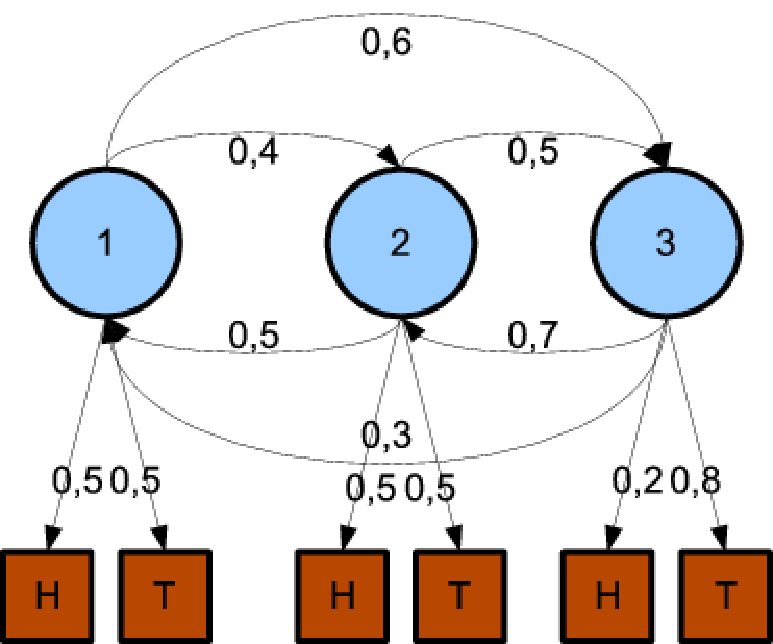
\includegraphics[width=.8\linewidth]{hmm-coins}
  
\end{frame}

% ------------------------------------------------------------

\begin{frame} \frametitle{Definitions}

  We will use the following notation:
  \begin{itemize}
  \item $N$ --- the number of \emph{states} in the model
  \item $M$ --- the number of distinct \emph{observation symbols}
  \item $T$ --- the length of the \emph{observation sequence}
  \item $i_t$ --- the state in which we are at time $t$
  \item $V = \{V_1, \dotsc, V_M\}$ --- the set of observation symbols
  \item $\pi = \{\pi_i\}$ --- the probability of being in state $i$ at the
    beginning of the experiment, i.e. $\pi_i = P(i_1 = i)$
  \item $A = \{a_{ij}\}$ --- the probability of being in state $j$ at time
    $t+1$ given that we were in state $i$ at time $t$,
    i.e. $P(i_{t+1}=j|i_t=i)$
  \item $B = \{b_j(k)\}$ --- the probability of observing symbol $v_k$ given
    that we are in state $j$, i.e., $P(v_k \text{ at } t|i_t = j)$
  \item $O_t$ the observation symbol observed at time $t$
  \item $\lambda = (A, B, \pi)$ --- the \emph{Hidden Markov Model}
  \end{itemize}
  
\end{frame}

% ------------------------------------------------------------

\begin{frame} \frametitle{An example}

  Consider a set of $n$ urns, each containing marbles of $m$ different
  colors. We are randomly choosing an urn and randomly picking a marble from
  it. How do we model this as an HMM?
  \begin{itemize}
  \item What are the states?
  \item What are the observation symbols?
  \end{itemize}

\end{frame}

\begin{frame} \frametitle{An example (cont.)}

  \begin{itemize}[<+->]
  \item The model would represent the following sequence of events:
    \begin{enumerate}
    \item We choose one of the urns, according to probability distribution
      $\pi$
    \item We choose a marble from that urn, according to probability
      distribution $B$
      \label{item:1}
      \begin{itemize}
      \item At this moment we are at time $t_1$, state $i_1$, and observed
        symbol $O_1$
      \item After the next step we will be at time $t_2$
      \end{itemize}
    \item We choose another urn, according to probability distribution $A$
    \item Repeat from step~\ref{item:1}, until we have made $T$ observations
      (i.e., t=$T$)
    \end{enumerate}
  \item The generated observation sequence will be $O_1, O_2, \dotsc, O_T$.
  \end{itemize}

\end{frame}

% ------------------------------------------------------------

\begin{frame} \frametitle{Three Problems for HMMs}

  \begin{enumerate}
  \item Given the model $\lambda = (A, B, \pi)$, compute $P(O|\lambda)$
    \begin{itemize}
    \item I.e., compute the probability of observing a given sequence
    \item Applications in \emph{language modeling, spelling correction}, $\ldots$
    \end{itemize}
  \item Given the model $\lambda = (A, B, \pi)$, choose a state sequence
    $I=i_1,i_2, \dotsc, i_T$ such that $P(O,I|\lambda)$ is maximized, for a
    given observation sequence $O=O_1,O_2,\dotsc,O_T$
    \begin{itemize}
    \item I.e., compute the most likely sequence of states to have generated an observation sequence (i.e., \emph{decoding})
    \item Applications in \emph{information extraction} (e.g., chunking, named entity recognition, $\ldots$)
    \end{itemize}
  \item Adjust the model parameters $\lambda = (A,B,\pi)$ such that
    $P(O|\lambda)$ or $P(O,I|\lambda)$, is maximized
    \begin{itemize}
    \item I.e., based on a series of observations and/or state sequences,
      compute the HMM
     \item Learning model parameters from annotated data
    \end{itemize}
  \end{enumerate}
  
\end{frame}

% ------------------------------------------------------------

\section{Probability of an Observation Sequence}

\begin{frame} \frametitle{Computing the Probabilities}

  \begin{itemize}
  \item We know that
    \begin{displaymath}
      P(O|\lambda) = \sum_I P(O|I,\lambda) P(I|\lambda)
    \end{displaymath}
  \item and since
    \begin{eqnarray*}
      P(O|I,\lambda) & = & b_{i_1}(O_1)b_{i_2}(O_2) \dotsb b_{i_T}(O_T) \\
      P(I|\lambda) & = & \pi_{i_1}a_{i_1i_2}a_{i_2i_3} \dotsb a_{i_{T-1}i_T}
    \end{eqnarray*}
  \item we have that
  \end{itemize}
  \begin{block}{}
    \begin{displaymath}
      P(O|\lambda) = \sum_I \pi_{i_1}b_{i_1}(O_1)a_{i_1i_2}b_{i_2}(O_2) \dotsb a_{i_{T-1}i_T}b_{i_T}(O_T)
    \end{displaymath}
  \end{block}
  
\end{frame}

% ------------------------------------------------------------

\begin{frame} \frametitle{The Problem}

  \begin{block}{}
    \begin{displaymath}
      P(O|\lambda) = \sum_I \pi_{i_1}b_{i_1}(O_1)a_{i_1i_2}b_{i_2}(O_2) \dotsb a_{i_{T-1}i_T}b_{i_T}(O_T)
    \end{displaymath}
  \end{block}

  \begin{itemize}
  \item Computing each summand requires $2T-1$ multiplications
  \item The are $N^T$ possible state sequences
  \item Thus, the complexity is $O(2TN^T)$: \emph{unfeasible}
  \item However, there is a more efficient way of computing $P(O|\lambda)$: the
    \emph{forward/backward procedure}
  \end{itemize}
  
\end{frame}

% ------------------------------------------------------------

\begin{frame} \frametitle{The Forward Procedure}

  \begin{itemize}
  \item Consider the \emph{forward variable} $\alpha_t(i)$, defined as:
    \begin{displaymath}
      \alpha_t(i) = P(O_1, O_2, \dotsc, O_t, i_t = i|\lambda)
    \end{displaymath}
    i.e., the probability of a partial observation sequence (until time $t$)
    that ends in state $i$
  \item $\alpha_t(i)$ can be computed as follows:
    \begin{enumerate}
    \item Compute the probability of starting in state $i$ and observing $O_1$:
      $\alpha_1(i)$
    \item For time $t+1$ compute the probability of reaching a state $j$ and
      observing $O_{t+1}$, knowing that we already computed all probabilities
      for all times $\leq t$
    \item The final probability (at time $T$) will be the sum of all
      probabilities for each possible ending state $i$:  $\alpha_T(i)$
    \end{enumerate}
  \end{itemize}
  
\end{frame}

% ------------------------------------------------------------

\begin{frame} \frametitle{Computing The Forward Procedure}

  \begin{block}{}
    \begin{enumerate}[<+->]
    \item Initial step:
      \begin{displaymath}
        \alpha_1(i) = \pi_ib_i(O_1) \; , \; 1 \leq i \leq N
      \end{displaymath}
    \item For $t = 1, 2, \dotsc, T-1$, $1 \leq j \leq N$
      \begin{displaymath}
        \alpha_{t+1}(j) = \left[ \sum_{i=1}^N \alpha_t(i)a_{ij} \right]b_j(O_{t+1})
      \end{displaymath}
    \item Thus, we have that:
      \begin{displaymath}
        P(O|\lambda) = \sum_{i=1}^N \alpha_T(i)
      \end{displaymath}
    \end{enumerate}
  \end{block}
  
\end{frame}

% ------------------------------------------------------------

\begin{frame} \frametitle{Time Complexity}

  \begin{itemize}
  \item Step 1 requires $N$ multiplications
  \item Step 2 requires $N+1$ multiplications. This is performed for all $N$
    states and $T-1$ times, yielding $(N+1)N(T-1)$ multiplications
  \item Step 3 requires only to sum the computed values
  \item Thus, the time complexity is \emph{$O(N^2T)$}
  \end{itemize}
  
\end{frame}

% ------------------------------------------------------------

\begin{frame} \frametitle{Backward Procedure}

  \begin{itemize}
  \item A similar procedure can be applied \textit{moving backwards}
  \item Consider the backward variable $\beta_t(i)$, defined as:
    \begin{displaymath}
      \beta_t(i) = P(O_{t+1}, O_{t+2}, \dotsc, O_T|i_t = i, \lambda)
    \end{displaymath}
    i.e., the probability of observing a partial sequence starting at time
    $t+1$ and state $i$
  \item $\beta_t(i)$ can also be computed as follows:
    \begin{enumerate}
    \item
      \begin{displaymath}
        \beta_T(i) = 1 \; , \; 1 \leq i \leq N
      \end{displaymath}
    \item For $t = T-1, T-2, \dotsc, 1$, $1 \leq i \leq N$, we have
      \begin{displaymath}
        \beta_t(i) = \sum_{j=1}^N a_{ij}b_j(O_{t+1})\beta_{t+1}(j)
      \end{displaymath}
    \item Thus, we have that:
      \begin{displaymath}
        P(O|\lambda) = \sum_{i=1}^N \pi_ib_i(O_1)\beta_1(i)
      \end{displaymath}
    \end{enumerate}
  \end{itemize}
  
\end{frame}

% ------------------------------------------------------------

\section{Probability of a Sequence of States}

\begin{frame} \frametitle{The Decoding Problem}

  \begin{itemize}
  \item We want to find a sequence of states $I = i_1, i_2, \dotsc, i_T$ such
    that the probability of observing a sequence $O = O_1, O_2, \dotsc, O_T$ is
    greater than for any other sequence
  \item I.e., Find $I$ that maximizes $P(O,I|\lambda)$
    \begin{displaymath}
      \arg \max_{\{i_t\}_{t=1}^T} P(O,i_1, i_2, \dotsc, i_T|\lambda)
    \end{displaymath}
  \item This can be computed using the \emph{Viterbi Algorithm}
  \end{itemize}
  
\end{frame}

% ------------------------------------------------------------

\begin{frame} \frametitle{The Viterbi Algorithm}

  \begin{itemize}
  \item We know that
    \begin{eqnarray*}
      P(O,I|\lambda) & = & P(O|I,\lambda)P(I|\lambda) \\
                     & = & \pi_{i_1}b_{i_1}(O_1)a_{i_1i_2}b_{i_2}(O_2) \dotsb a_{i_{T-1}i_T}b_{i_T}(O_T)
    \end{eqnarray*}
  \item Thus, we can define
    \begin{displaymath}
      U(i_1, i_2, \dotsc, i_T) = 
        - \left[ \ln\big(\pi_{i_1}b_{i_1}(O_1)\big) +
                 \sum_{t=2}^T \ln\big(a_{i_{t-1}i_t}b_{i_t}(O_t)\big)
         \right]
    \end{displaymath}
  \item so that
    \begin{displaymath}
      P(O,I|\lambda) = \exp(-U(i_1, i_2, \dotsc, i_T))
    \end{displaymath}
  \item and our problem becomes
    \begin{block}{}
      \begin{displaymath}
        \arg \min_{\{i_t\}_{t=1}^T} U(i_1, i_2, \dotsc, i_T)
      \end{displaymath}
    \end{block}
  \end{itemize}
  
\end{frame}

% ------------------------------------------------------------

\begin{frame} \frametitle{The Viterbi Algorithm (cont.)}

  \begin{itemize}
  \item We can view the term $-\ln(a_{i_ji_k}b_{i_k}(O_t))$ as the cost of going
    from state $i_j$ to state $i_k$ at time $t$
  \item The Viterbi Algorithm is a \emph{dynamic programming} approach to
    compute the path of least cost
  \item The total cost of a path is the sum of the weights on the edges we
    cross
    \begin{itemize}
    \item Note that this is equivalent to multiplying the probabilities
    \end{itemize}
  \end{itemize}
  
\end{frame}

% ------------------------------------------------------------

\begin{frame}[allowframebreaks] \frametitle{Computing the Viterbi Algorithm}

  \begin{itemize}
  \item Let $\delta_t(i)$ be the accumulated weight at state $i$ and time $t$
  \item Let $\psi_t(j)$ be the state at time $t-1$ with the lowest cost
    transition to state $j$ at time $t$
  \end{itemize}

  \begin{enumerate}
  \item Initialization, for $1 \leq i \leq N$:
    \begin{eqnarray*}
      \delta_1(i) & = & -\ln(\pi_i)-\ln(b_i(O_1)) \\
      \psi_1(i) & = & 0
    \end{eqnarray*}
  \item Recursive computation, for $2 \leq t \leq T$, $1 \leq j \leq N$:
    \begin{eqnarray*}
      \delta_t(j) & = & \min_{1\leq i \leq N}[\delta_{t-1}(i)-\ln(a_{ij})]-\ln(b_j(O_t)) \\
      \psi_t(j) & = & \underset{1\leq i \leq N}{\operatorname{arg\,min}}[\delta_{t-1}(i)-\ln(a_{ij})]
    \end{eqnarray*}
  \item Termination:
    \begin{eqnarray*}
      P^* & = & \min_{1 \leq 1 \leq N}[\delta_T(i)]\\
      q_T^* & = & \underset{1\leq i \leq N}{\operatorname{arg\,min}}[\delta_T(i)]
    \end{eqnarray*}
  \item Trace back, for $t = T, T-1, T-2, \dotsc, 1$:
    \begin{displaymath}
      q_t^* = \psi_{t+1}(q_{t+1}^*)
    \end{displaymath}
  \end{enumerate}

  \begin{itemize}
  \item $Q^* = \{q_1^*, q_2^*, \dotsc, q_T^*\}$ is the optimal state sequence
  \item $\exp(-P^*)$ is the optimized probability for the state sequence
  \end{itemize}

  \vspace{2ex}

  \begin{itemize}
  \item Complexity: $O(N^2T)$
  \end{itemize}
  
\end{frame}

% ------------------------------------------------------------

\begin{frame} \frametitle{An Example Computation}

  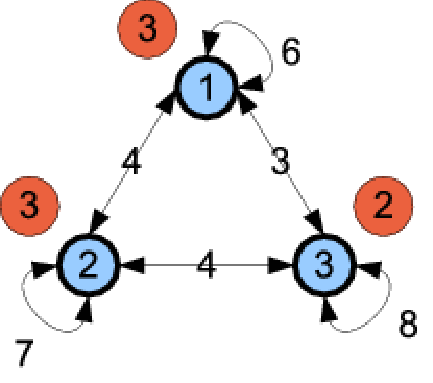
\includegraphics[scale=.6]{viterbi1}\\[-2\baselineskip]
  \hfill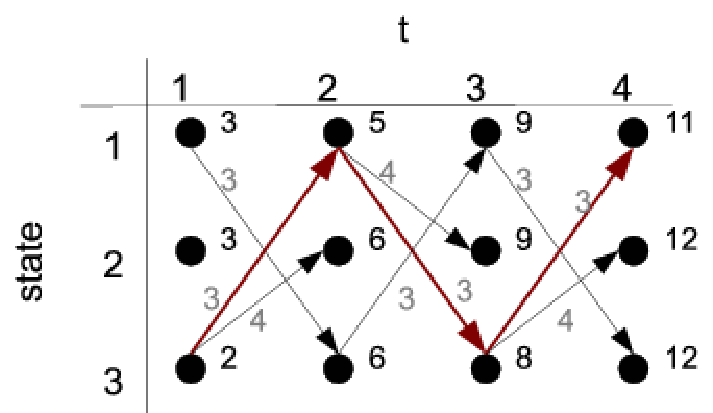
\includegraphics[scale=.6]{viterbi2}
  
\end{frame}

\begin{frame} \frametitle{Notes}
  \begin{itemize}
  \item The Viterbi algorithm can be used with HMMs, and also with other sequential classification models (e.g., structured Perceptrons, CRFs, neural network approaches, $\ldots$)
  
  \item Other {\it decoding} approaches are also frequently used in practice, one example being \emph{posterior decoding} 
  % http://web.mit.edu/6.047/book-2012/Lecture08_HMMSII/Lecture08_HMMSII_standalone.pdf
  % http://stellar.mit.edu/S/course/6/fa12/6.047/courseMaterial/topics/topic2/lectureNotes/Lecture07_HMMsIIb_6up/Lecture07_HMMsIIb_6up.pdf
  \begin{itemize}
  \item Determine, independently for every symbol $O_t$, the most probable state using the forward/backward procedure
  \item Often more effective when several concurring paths have similar probabilities
  \end{itemize}

  \item Some practical implementations of Information Extraction tools, leveraging sequential classification models, rely on methods such as \emph{beam search} to find an approximate solution to the problem of finding state sequences % https://en.wikipedia.org/wiki/Beam_search

  \end{itemize}
\end{frame}

% ------------------------------------------------------------

\section{Learning the Model}

\begin{frame} \frametitle{Learning HMMs}
  
  \begin{itemize}
  \item In a \emph{supervised setting}, we use the training data to estimate
      the probabilities
  \item Transition probabilities
    \begin{block}{} \scriptsize
      \begin{displaymath}
        \hat{P}(i \rightarrow i') = \frac{c(i \rightarrow i')}{\sum_{s \in I}c(i \rightarrow s)}
      \end{displaymath}
    \end{block}

  \item Emission probabilities
    \begin{block}{} \scriptsize
      \begin{displaymath}
        \hat{P}(i \uparrow o) = \frac{c(i \uparrow o)}{\sum_{\rho \in O}c(i \uparrow \rho)}
      \end{displaymath}
    \end{block}
  \end{itemize}

  \vspace{1.0ex}

  { \scriptsize
  \begin{itemize}
  \item $c(i \rightarrow i')$ is the number of times there is a transition from state $i$ to state $i'$ (in a training set)
  \item $c(i \uparrow o)$ counts the number of times symbol $o$ is observed in state $i$ (in a training set)
  \item The \emph{estimation of beginning probabilities} is similar to that of transition probabilities, but we count the number of times there is a transition from the start (i.e., the beginning of a training sequence) to a state $i$
  \end{itemize}
  }
\end{frame}

% ------------------------------------------------------------

\begin{frame} \frametitle{Improving Probability Estimates}
  
  \begin{itemize}
  \item Problem: sparse training data causes poor probability estimates
    \begin{itemize}
    \item E.g., unseen symbols have emission probabilities of zero
    \end{itemize}
  \item Solution: use probability smoothing techniques
    \begin{itemize}
    \item Laplace smoothing
    \item Absolute discounting
    \item $\ldots$
    \end{itemize}
  \end{itemize}

\end{frame}

% ------------------------------------------------------------

\begin{frame} \frametitle{Laplace Smoothing}
  
  \begin{itemize}
  \item Adds 1 to every count of occurrences
  \item Moves all estimates towards the uniform distribution
  \item All unseen words will have equal probability
  \end{itemize}

  An example:
  \begin{displaymath}
    \hat{P}(i \uparrow o) = \frac{c(i \uparrow o) + 1}{\sum_{\rho \in
        O}c(i \uparrow \rho) + |O|}
  \end{displaymath}

\end{frame}

% ------------------------------------------------------------

\begin{frame} \frametitle{Absolute Discounting}
  
  \begin{itemize}
  \item Localized (per state) smoothing
  \item Appropriate if zero probabilities vary from state to state
  \item Subtracts a fixed discount $0 < d < 1$ from all symbols with count $>0$
  \item The total discounted value is distributed by the remaining symbols
  \end{itemize}

  An example:
  \begin{displaymath}
    \hat{P}(i \uparrow o) = 
    \left\{
    \begin{array}{ll}
      \frac{c(i \uparrow o)-d}
           {\sum_{\rho \in O}c(i \uparrow \rho)} &
                 \text{if $c(i \uparrow o) > 0$ }\\[2ex]
      \frac{d(|O|-|Z_q|)}{|Z_q|*\sum_{\rho \in O}c(i \uparrow \rho)} &
         \text{if $c(i \uparrow o) = 0$ }
    \end{array}
    \right.
  \end{displaymath}
  where $|Z_q|$ is the number of symbols with zero count in state $i$.

\end{frame}



\begin{frame} \frametitle{Unsupervised Learning of HMMs}

  \begin{itemize}
  \item We want to train an HMM model with a set of \emph{example observation
        sequences} such that, when a similar sequence is discovered later the
      model is able to identify it.
  \item Most well known method
      \begin{itemize}
      \item \emph{Baum-Welch} algorithm
      \end{itemize}
  \item Other methods exist
      \begin{itemize}
      \item E.g. \emph{Segmental K-means}
      \end{itemize}
  \end{itemize}
  
\end{frame}

% ------------------------------------------------------------

\begin{frame}
    \frametitle{The Baum-Welch Method}
    \begin{itemize}
    \item Assume an initial model $\lambda$
        \begin{itemize}
        \item Can be constructed in any way (e.g. randomly)
        \end{itemize}
    \item Maximizes $P(O|\lambda)$ by adjusting $\lambda$
        \begin{itemize}
        \item Called the \emph{maximum likelihood criterion}
        \end{itemize}
    \end{itemize}
\end{frame}

\begin{frame}
    \frametitle{Probability of Visiting a State}
    \begin{itemize}
    \item Let
        \begin{displaymath}
            \gamma_t(i) = P(i_t = t|O,\lambda)
        \end{displaymath}
        i.e. the probability of being in state $i$ at time $t$ given the
        observation sequence $O$ and the model $\lambda$
    \item Applying Bayes rule:
        \begin{displaymath}
            \gamma_t(i) = \frac{P(i_t=i,O)}{P(O|\lambda)} = \frac{\alpha_t(i)\beta_t(i)}{P(O|\lambda)}
        \end{displaymath}
        where $\alpha_t(i)$ is computed as in the Forward procedure and
        $\beta_t(i)$ is computed as in the Backward procedure
    \end{itemize}
\end{frame}

% t ( i ) accounts for O 1 ,. . . , O t and state i at time t , and t ( i ) accounts for O t +1 ,. . . , O T given state i at time t .

\begin{frame}
    \frametitle{Probability of Transitioning}
    \begin{itemize}
    \item Let
        \begin{displaymath}
            \xi_t(i) = P(i_t = i, i_{t+1} = j|O,\lambda)
        \end{displaymath}
        i.e. the probability of being in state $i$ at time $t$ and making a
        transition to state $j$ at time $t + 1$, given the observation sequence
        $O$ and the model $\lambda$
    \item Applying Bayes rule:
        \begin{multline*}
            \xi_t(i) = \\
            \frac{P(i_t = i, i_{t+1} = j,O|\lambda)}{P(O|\lambda)} = \\
            \frac{\alpha_t(i)a_{ij}b_j(O_{t+1})\beta_{t+1}(j)}{P(O|\lambda)}
        \end{multline*}
    \end{itemize}
\end{frame}

% \begin{frame}
%     \frametitle{Probability of Transitioning (cont.)}
%     \small
%     Since
%     \begin{multline*}
%         P(i_t = i, i_{t+1} = j,O|\lambda) = \\
%         P(i_t = i, i_{t+1} = j, O_1, \ldots, O_t, O_{t+1} \ldots, O_{T}|\lambda) = \\
%         P(i_t = i, O_1, \ldots, O_t|\lambda)P(i_{t+1} = j, O_{t+1} \ldots, O_{T}|\lambda) = 
%     \end{multline*}
%     and
%     \begin{displaymath}
%         P(i_t = i, O_1, \ldots, O_t|\lambda) = \alpha_t(i)
%     \end{displaymath}
%     and
%     \begin{multline*}
%         P(i_{t+1} = j, O_{t+1} \ldots, O_{T}|\lambda) = \\
%         P(i_{t+1} = j, O_{t+1}|\lambda)P(O_{t+1} \ldots, O_{T}|i_{t+1} = j, \lambda) = \\
%         a_{ij}b_j(O_{t+1})\beta_{t+1}(j)
%     \end{multline*}
%     we have that \normalsize
%     \begin{displaymath}
%         \xi_t(i,j) = \frac{\alpha_t(i)a_{ij}b_j(O_{t+1})\beta_{t+1}(j)}{P(O|\lambda)}
%     \end{displaymath}
% \end{frame}

\begin{frame}
    \frametitle{Expected Number of Transitions}
    Expected number of visits to state $i$:
    \begin{displaymath}
        \sum_{t=1}^{T}\gamma_t(i)
    \end{displaymath}
     Expected number of transitions from state $i$:
    \begin{displaymath}
        \sum_{t=1}^{T-1}\gamma_t(i)
    \end{displaymath}
     Expected number of transitions from state $i$ to state $j$:
    \begin{displaymath}
        \sum_{t=1}^{T-1}\xi_t(i,j)
    \end{displaymath}
\end{frame}

% If we sum up t ( i ) from t = 1 to T we get a quantity which can be viewed as
% the expected number of times state i is visited or if we sum up only up to T
% ? 1 then we shall get the expected number of transitions out of state i (as
% no transition is made at t = T ). Similarly if  t ( i,j ) be summed up from
% t = 1 to T ? 1, we shall get the expected number of transitions from state i
% to state j .

\begin{frame}
    \frametitle{Baum-Welch Re-Estimation Formulas}
    The new model paramters $\hat{\lambda}=(\hat{A},\hat{B},\hat{\pi})$ can be
    computed as:
    \begin{displaymath}
        \hat{\pi}_i = \gamma_1(i)
    \end{displaymath}\\
    \begin{displaymath}
        \hat{a}_{ij} = \sum_{t=1}^{T-1}\xi_t(i,j) \Bigg/ \sum_{t=1}^{T-1}\gamma_t(i)
    \end{displaymath}
    \vfill
    \begin{displaymath}
        \hat{b}_i(k) = \sum_{t=1 | O_t=k}^T\gamma_t(i) \Bigg/ \sum_{t=1}^T\gamma_t(i)
    \end{displaymath}
\end{frame}

% https://en.wikipedia.org/wiki/Baum%E2%80%93Welch_algorithm#Example
% slide 15 http://www.biostat.jhsph.edu/bstcourse/bio638/notes/HMMs_BaumWelch.pdf

\begin{frame}
    \frametitle{Multiple Observation Sequences}
    For multiple observation sequences, sum $\xi_t(i,j)$ and $\gamma_t(i)$ and
    over all sequences:
    \begin{displaymath}
        \hat{\pi}_i = \sum_{O}\gamma_1(i)
    \end{displaymath}\\
    \begin{displaymath}
        \hat{a}_{ij} = \sum_{O}\sum_{t=1}^{T-1}\xi_t(i,j) \Bigg/ \sum_{O}\sum_{t=1}^{T-1}\gamma_t(i)
    \end{displaymath}
    \vfill
    \begin{displaymath}
        \hat{b}_i(k) = \sum_{O}\sum_{t=1 | O_t=k}^T\gamma_t(i) \Bigg/ \sum_{O}\sum_{t=1}^T\gamma_t(i)
    \end{displaymath}
    The final values will then have to be normalized.
\end{frame}

% https://stackoverflow.com/questions/17125519/how-do-i-have-to-train-a-hmm-with-baum-welch-and-multiple-observations
% http://citeseerx.ist.psu.edu/viewdoc/download?doi=10.1.1.335.1457&rep=rep1&type=pdf

% ------------------------------------------------------------

\section{Other Sequential Classification Models}

\begin{frame} \frametitle{Other Models}
  
  \begin{itemize}
  \item Structured Perceptron
  \item Conditional Random Fields
  \item Recurrent or Convolutional Deep Neural Networks
  \item $\ldots$
  \end{itemize}
 
\end{frame}

\begin{frame} \frametitle{Restructuring HMMs With Features (1)}
\begin{itemize}
\item In a regular HMM, we have that:
\begin{eqnarray*}
      P(O,I|\lambda) & = & P(O|I,\lambda)P(I|\lambda) \\
                     & = & \pi_{i_1}b_{i_1}(O_1)a_{i_1,i_2}b_{i_2}(O_2) \dotsb a_{i_{T-1}i_T}b_{i_T}(O_T)
\end{eqnarray*}

\item Considering the log likelihood:
\begin{eqnarray*}
\log\left(P(O,I|\lambda)\right) & = & \log\left(\pi_{i_1}\right) + \log\left(b_{i_1}(O_1))\right) + \\
                                &   &\log\left(a_{i_1i_2})\right) + \log\left(b_{i_2}(O_2))\right) + \dotsb + \\
                                &   & \log\left(a_{i_{T-1}i_T})\right) + \log\left(b_{i_T}(O_T))\right)
\end{eqnarray*}

\item Considering scores, and assuming that $W(t,O_t) = \log(a_{i_{t-1}i_t}) + \log(b_{i_{t}}(O_t))$, we have:

\begin{displaymath}
S(O,I|\lambda) = \sum_{t=1}^{T} W(t,O_t)
\end{displaymath}
\end{itemize}
\end{frame}

\begin{frame} \frametitle{Restructuring HMMs With Features (2)}
\begin{itemize}
\item In the previous example, we saw how to express a model equivalent to an HMM through scoring functions $W(t,Ot)$ that leverage state transitions between adjacent positions in the sequence (i.e., from $t-1$ to $t$), and symbol emissions for position $t$ of the input sequence.

\item Scoring functions can also be written as a linear combination of $K$ different features, again describing state transitions between adjacent positions in the sequence, and symbol emissions for position $t$ of the input sequence.

\item In information extraction applications, we want to find the state sequence I that satisfies:
{\scriptsize
\begin{displaymath}
\hat{I} = \arg \max_I S(O,I|\lambda) = \arg \max_I \sum_{t=1}^T \sum_{k=1}^K\lambda_kf_k(I_t, I_{t-1}, O_t)
\end{displaymath} }
\end{itemize}

\end{frame}

\begin{frame} \frametitle{Structured Perceptron (just a hint)}
  
   \begin{itemize}
   \scriptsize
   \item Simple discriminative model that enables exploring features representing symbols (e.g., {\it capital letters denote nouns?})
   \item Viterbi algorithm now considers feature weights for computing costs
   \item High dimensional feature vector represents each possible transition/emission (e.g., one feature per emission/transition in a HMM)
   \item Update feature weights incrementally, so as to increase/decrease score of correct/incorrect labellings
   \end{itemize}
  
   \begin{block}{}
   \begin{enumerate}
   \item Create feature map and set initial feature weights $w$
   \item For $\epsilon$ iterations, and for each labeled pair $\{O,I\}$ in the training data
   \begin{enumerate}
   \item Compute $\hat{I}$ for the observation sequence $O$, using the Viterbi algorithm and the feature vector $w$
   \item If $I=\hat{I}$ do not update the model, else
   \begin{enumerate}
   \item Compute the feature vector $f$ for the pair $\{O,I\}$
   \item Compute the feature vector $\hat{f}$ for the pair $\{O,\hat{I}\}$
   \item Update the feature vector: $w = w + f - \hat{f}$
   \end{enumerate}
   \end{enumerate}
   \end{enumerate}
   \end{block}
 \end{frame}
 
\begin{frame}
\frametitle{Guarantees with Perceptron Learning}
Simple additive update seems intuitive, but do we have any guarantees? Collins (2002) has some proofs showing that:
\begin{itemize}
\item If the data is separable with some margin, then the algorithm will converge on weights which give zero error on the training data
\item If the training data is not separable, but “close” to being separable, then the algorithm will make a small number of mistakes (on the training data)
\item If the algorithm makes a small number of errors on the training data, it is likely to generalise well to unseen data
\end{itemize}
Reference: {\it Michael Collins, Discriminative Training Methods for Hidden Markov Models: Theory and Experiments with Perceptron Algorithms, 2002}
\end{frame}

 \begin{frame}
     \frametitle{Linear-Chain Conditional Random Fields (1)}
     \centering
     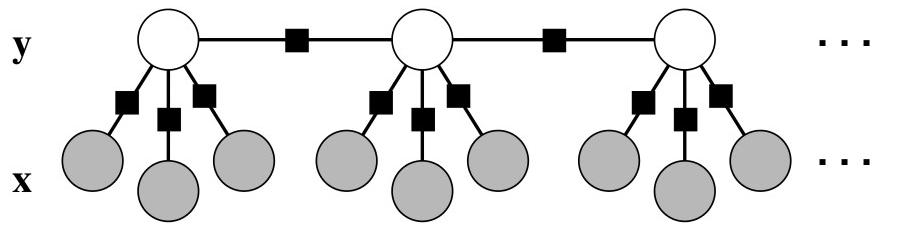
\includegraphics[width=.9\linewidth]{crf}
     \begin{displaymath}
         P(I|O) = \frac{1}{Z(O)}\exp\left\{\sum_{t=1}^T \sum_{k=1}^K\lambda_kf_k(I_t, I_{t-1}, O_t)\right\}
     \end{displaymath}
     \begin{itemize}
     \item Inference with the Viterbi algorithm
     \item Infering the parameters by maximum likelihood learning, e.g., through generalized iterative scaling or through gradient descent algorithms
     \end{itemize}
\end{frame}

 \begin{frame}
     \frametitle{Linear-Chain Conditional Random Fields (2)}
     \begin{itemize}
     \item Inference leverages the Viterbi algorithm to find the following argmax efficiently
	 \begin{eqnarray*}
         \arg \max_I P(I|O) & = &  \arg \max_I \exp\left\{\sum_{t=1}^T \sum_{k=1}^K\lambda_kf_k(I_t, I_{t-1}, O_t)\right\} \frac{1}{Z(O)} \\
		                    & = & \arg \max_I \left\{\sum_{t=1}^T \sum_{k=1}^K\lambda_kf_k(I_t, I_{t-1}, O_t)\right\} - \log \left( \frac{1}{Z(O)} \right) \\
							& = & \arg \max_I \left\{\sum_{t=1}^T \sum_{k=1}^K\lambda_kf_k(I_t, I_{t-1}, O_t)\right\} 
     \end{eqnarray*}
     \item Computing the normalisation term $Z(O)$ can be made efficiently with the forward procedure
	 \item Training is a convex optimization problem, e.g. solved through generalized iterative scaling and computing the feature expectations (denominator) through the forward-backward procedure
%	 \begin{displaymath}
%     \lambda_i^{[k+1]} = \lambda_i^{[k]} + \frac{1}{Z(O)} \log\left \frac{ \sum_{t=1}^T f_k(I_t, I_{t-1}, O_t)  }{ \sum_I' P(I|O,\lambda^{[k]})  \sum_{t=1}^T f_k(I'_t, I'_{t-1}, O_t) }  \right)
%	 \end{displaymath}
     \end{itemize}
\end{frame}

% ------------------------------------------------------------

\finalframe{\Large{Questions?}}

% ------------------------------------------------------------

\finalframe{\Large{Extra Credits}}

\begin{frame} \frametitle{The Segmental K-means Algorithm}

  \begin{itemize}
  \item Segmental K-means adjusts the parameters $\lambda = (A, B, \pi)$ to
    maximize $P(O,I|\lambda)$, where $I$ is the optimal sequence of states for
    observation sequence $O$
  \item Idea: evolve from $\lambda^k$ to $\lambda^{k+1}$ such that
    $P(O,I^*_k|\lambda^k) \leq P(O,I^*_{k+1}|\lambda^{k+1})$
  \item $I^*_k$ is the optimal state sequence for $O = O_1, O_2, \dotsc, O_T$
    and $\lambda_k$
  \item Function $P(O,I^*|\lambda) = \max_I P(O,I|\lambda)$ is called the
    \emph{state optimized likelihood function}
  \item This optimization criterion is called \emph{maximum state optimized
      likelihood criterion}
  \end{itemize}
  
\end{frame}

% ------------------------------------------------------------

\begin{frame} \frametitle{The Segmental K-means Algorithm (cont.)}

  Basic assumptions:
  \begin{itemize}
  \item We have a set of $w$ observation sequences available (\emph{training
      sequences})
  \item Each training sequence $O = O_1, O_2, \dotsc, O_T$ consists of $T$
    observation symbols
  \item Each observation symbol $O_i$ is a \emph{vector of $D$ ($\geq 1$) dimensions}
  \end{itemize}
  
\end{frame}

% ------------------------------------------------------------

\begin{frame}[allowframebreaks] \frametitle{Computing the Algorithm}

  \begin{enumerate}
  \item Randomly choose $N$ observation symbols; assign each of the $wT$
    training symbols to the closest chosen symbol (e.g., using Euclidean distance)
  \item Calculate the initial probabilities and transition probabilities:
    \begin{itemize}
    \item For $1 \leq i \leq N$:
      \begin{displaymath}
        \hat{\pi}_i = \frac{ \text{Number of occurrences of $\{O_1 \in i\}$} }
                           { \text{Total number of occurrences of $O_1$ (i.e., $w$)} }
      \end{displaymath}
    \item For $1 \leq i \leq N$, $1 \leq j \leq N$:
      \begin{displaymath}
        \hat{a}_{ij} = \frac{ \text{Number of occurrences of $\{O_t \in i$ and $O_{t+1} \in j\}, \forall t$} }
                           { \text{Total number of occurrences of $O_t \in i, \forall t$} }
      \end{displaymath}
    \end{itemize}
    \label{item:2}
  \item Compute mean and covariance matrix of each state. For $1 \leq i \leq N$:
    \begin{eqnarray*}
      \hat{\mu}_i & = & \frac{1}{N_i}\sum_{O_t \in i} O_t \\
      \hat{V}_i & = & \frac{1}{N_i}\sum_{O_t \in i}(O_t - \hat{\mu}_i)^T(O_t - \hat{\mu}_i)
    \end{eqnarray*}
  \item Calculate the probability distribution of each symbol in each state:
    \begin{displaymath}
      \hat{b}_i(O_t) = \frac{1}{((2\pi)^{D/2}|\hat{V}_i|^{1/2}}
                       \exp[-\frac{1}{2}(O_t-\hat{\mu}_i)\hat{V}_i^{-1}(O_t-\hat{\mu}_i)^T]
    \end{displaymath}
    \begin{itemize}
    \item We are assuming a Gaussian distribution. Others could be used.
    \end{itemize}
  \item Find the optimal state sequence $I^*$ for each training sequence, using
    $\hat{\lambda}_i = (\hat{A}_i,\hat{B}_i,\hat{\pi}_i)$; reassign $O_t$ (of
    the $k$-th training sequence) to state $i$ iff $i_t^*$ (of the $k$-th
    training sequence) is $i$
    \begin{itemize}
    \item For instance: if $O_2$ of the 5th sequence was in state $3$, and in
      $I^*$ (for the 5th training sequence) we have that $i^*_2$ is 4, we
      assign $O_2$ of the 5th sequence to state 4.
    \end{itemize}
  \item If any symbol was reassigned, repeat from step~\ref{item:2}, otherwise
    stop.
  \end{enumerate}

  \vspace{2ex}

  \begin{itemize}
  \item It can be proved that the algorithm converges to the state-optimized likelihood function for many different observation probability distributions
  \end{itemize}
  
\end{frame}

\end{document}

%%% Local Variables: 
%%% mode: latex
%%% TeX-master: t
%%% End: 
